\chapter{Lecture 19 - Fourier-Bessel Series Expansions}
\label{ch:lec19}
\section{Objectives}
\begin{itemize}
\item Present the parametric Bessel equation as a Sturm-Liouville problem and derive the orthogonality relation.
\item Do an example to show a Fourier-Bessel expansion of a function.
\item Demonstrate use of the MATLAB function \lstinline{besselzero()}.
\end{itemize}

\section{Parametric Bessel Equation}
The parametric Bessel equation is a second-order linear, homogeneous differential equation that also fits within Sturm-Liouville theory.  As a reminder, the equation is:
\begin{equation*}
x^2u^{\prime \prime} + xu^{\prime} + \left(\alpha^2x^2-\nu^2\right)u = 0
\end{equation*}
and the general solution is given by:
\begin{equation*}
u(x) = c_1J_{\nu}(\alpha x) + c_2Y_{\nu}(\alpha x)
\end{equation*}

\noindent The solutions, $J_{\nu}(\alpha x)$ and $Y_{\nu}(\alpha x)$ are, of course, linearly independent but they also are orthogonal with respect to some weight function $p(x)$.  We can use them to construct an orthogonal function expansion in exactly the same way we did with Fourier series.  That is what we will do in this lecture.  To accomplish this we want to put the parametric Bessel equation in self-adjoint form and we will proceed in this effort just as we did in the last lecture.

\vspace{0.5cm}

\noindent Let us first put the parametric Bessel equation in standard form:\marginnote{It may not be clear immediately that $\lambda$ corresponds to values of $\alpha$ but that is the correct inference; when we do the orthogonal function expansion with Bessel functions it will be more clear why that is the case.}
\begin{align*}
a(x)u^{\prime \prime} + b(x)u^{\prime} + \left[c(x)+\lambda d(x) \right] u &= 0 \\
x^2u^{\prime \prime} + xu^{\prime} + \left[-\nu^2 + \alpha^2 x^2\right]u &=0
\end{align*}
so, $a(x) = x^2$, $b(x)=x$, $c(x) = -\nu^2$, and $d(x)=x^2$.

\vspace{0.25cm}

\noindent Next we will compute $r(x)$:
\begin{align*}
r(x) &= e^{\int \frac{b(x)}{a(x)} \ dx} \\
&= e^{\int \frac{x}{x^2} \ dx} \\
&= e^{\int \frac{1}{x} \ dx} \\
&= e^{\ln{x}} \\
&= x
\end{align*}

\vspace{0.25cm}

\noindent Now we compute $q(x)$:
\begin{align*}
q(x) &= \frac{c(x)}{a(x)}r(x) \\
&= \frac{-\nu^2}{x^2}x \\
&= -\frac{\nu^2}{x}
\end{align*}

\vspace{0.25cm}

\noindent Then $p(x)$:
\begin{align*}
p(x) &= \frac{d(x)}{a(x)}r(x) \\
&=\frac{x^2}{x^2}x \\
&= x
\end{align*}
So the self-adjoint form of the parametric Bessel equation is:\marginnote{Admittedly, the real reason why we want to do this is to obtain the weight function $p(x)$ which, in this case is $p(x)=x$.}
\begin{equation*}
\frac{d}{dx}\left[x u^{\prime} \right] + \left(-\frac{\nu^2}{x} + \alpha^2 x \right)u = 0
\end{equation*}
The corresponding orthogonality relation is shown in Equation \ref{eq:fb-ortho}:\marginnote{Like other Sturm-Liouville problems we will find that there are infinitely many distinct eigenvalues, $\lambda_n$, which for this equation we will refer to as $\alpha_n$.  Note the weight function $x$ now appears in the inner product.}
\begin{equation}
\int_{a}^{b}J_{\nu}(\alpha_n x) J_{\nu}(\alpha_m x) x \ dx = 0, \ \ n \ne m
\label{eq:fb-ortho}
\end{equation}
where $a$ and $b$ are the bounds of the interval on which orthogonality is expressed.

\vspace{0.5cm}

\noindent\textbf{Example:} Expand $f(x)=x, \ 0<x<3$, in a Fourier-Bessel series, using Bessel functions of order $\nu=1$ that satisfy the boundary condition $J_{1}(3\alpha)=0.$\marginnote[-1.25cm]{Remember that it is the \emph{boundary conditions} that allow us to determine the eigenvalues.}

\vspace{0.25cm}
\begin{marginfigure}
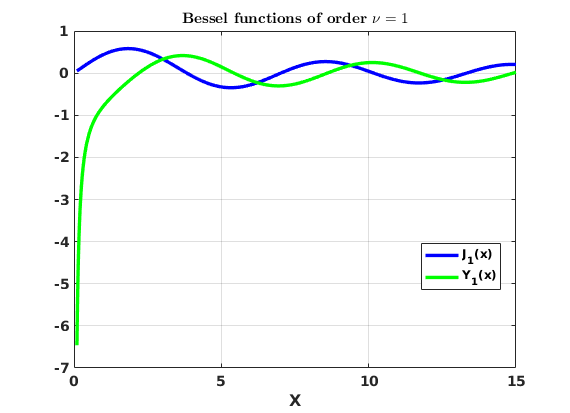
\includegraphics{lec19_bessel1_plot.png}
\label{fig:lec19-bessel}
\caption{Bessel functions of order 1.}
\end{marginfigure}
\noindent So what we want is:
\begin{equation*}
f(x) = x = \sum\limits_{n=1}^{\infty}c_n J_{1}\left(\alpha_n x\right)
\end{equation*}
Note that we omit Bessel functions of the second kind, $Y_n(x)$, because as is shown in the figure, they diverge to negative infinity as $x$ goes to zero.  This \emph{implicit boundary condition}, where one solution of the differential equation diverges at the problem boundary, often needs to be considered when solving boundary value problems.

The other boundary condition applies at $x=3$: $J_{1}(3\alpha_n) = 0$ or, put differently, we select the values of $\alpha_n$ such that $3\alpha_n$ is a root of $J_{1}(x)$.  While our plot of $J_1(x)$ does not extend out to infinity, it turns out that $J_1(x)$ has infinitely many roots and we need to find them.

\subsection{Interlude on Open-Source Software}
At some point in time in your life as an engineer it is inevitable that a problem will arise that you are not prepared to tackle yourself. The tools you have been given to do your job do not fully answer to the task at hand.  This is one such occasion.  We need to find the roots of $J_1(x)$.  \emph{You know} those values exist but you do not know what they are and it turns out that MATLAB does not (at this time) have any built-in functions to give you the roots of such functions either.\sidenote[][-2.0cm]{MATLAB \emph{does} have built-in functions to represent several types of Bessel functions; $J_{\nu}(x)$ and $Y_{\nu}(x)$ are represented, respectively, by \lstinline[style=myMatlab]{besselj(nu,x)} and \lstinline[style=myMatlab]{bessely(nu,x)}. We will learn about more Bessel functions in future lectures.}

\vspace{0.15cm}

\noindent Some options available to you include:
\begin{enumerate}
\item Go to the library and check out a book that tabulates some roots of $J_{1}(x)$---possibly also including scads of additional Bessel function lore\cite{bowman2012introduction}---and enter the desired roots by hand into your MATLAB code.
\item Implement an algorithm to find the roots of $J_1(x)$, possibly using a root-finding tool in MATLAB such as \lstinline[style=myMatlab]{fzero()} or \lstinline[style=myMatlab]{fsolve()}.
\item Find a third-party function or library that has already been written that solves the problem.
\end{enumerate}
In this case we will take the last option since, it turns out, someone \emph{has} already solved this problem for us\marginnote[-0.5cm]{The Fourier-Bessel expansion that we are learning about in this lecture is a standard element in the analytical methods repertoire; \emph{of course} someone else has already figured out how to find the roots of Bessel functions.} and it is a safe bet that they did a better job than what we would be prepared to do.  The MATLAB file exchange is an online repository where people can freely share code that they find useful and other users can look there in search of helpful code when needed.\sidenote{Note that a (free) MathWorks account is required to use the MATLAB file exchange.} 

\newthought{We have a lot} of experience with proprietary software.  From operating systems like Microsoft Windows or Apple's iOS to office productivity tools like Microsoft Word or Excel, to valuable and important engineering tools like MATLAB or COMSOL.  We also have experience with free software, such as many applications that you download onto your smartphones.  I want to write a few words in hopes of dispelling any negative connotations that you may have developed in relation to open-source software in comparison to proprietary software.
\begin{itemize}
\item Scientists and engineers of all types---not just computer scientists---write and share software.  Sometimes this software is open-source.  Online repositories like GitHub and GitLab are meant expressly for developing open-source software in a collaborative way and then sharing the results freely.
\item ``Open-source'' ensures the source code is available.  Sometimes the code is also free but that is not the essential part.\sidenote{To paraphrase the famous open-source software icon, Richard Stallman: free software means ``free speech,'' not ``free beer.''  But sometimes it is a lot like free beer too.}

\item Open-source software is a \emph{hugely} important contribution to science.  Some free and open-source tools include:
\begin{itemize}
\item The \LaTeX\ typesetting tools and almost all of the other software installed on the computer used to prepare this manuscript, including the Linux operating system.\sidenote{MATLAB is a notable exception to this list.  There is a free and open-source alternative called Octave. \url{https://octave.org/} }
\item Programming languages that have been a part of the scientific computing landscape for generations.  Some examples are Python, C++, Java and FORTRAN among others.
\item OpenMC\cite{ROMANO201590} - a powerful particle transport simulation tool similar to MCNP.
\item MOOSE - \underline{M}ulti-physics \underline{O}bject-\underline{O}riented \underline{S}imulation \underline{E}nvironment\cite{lindsay2022moose} which combines the open-source finite element library libMesh\cite{kirk2006libmesh} and the \underline{P}ortable, \underline{E}xtensible \underline{T}oolkit for \underline{S}cientific \underline{C}omputation (PETSc)\cite{petsc-user-ref} along with a host of other free, open-source libraries to create an enormously powerful and flexible tool-set that is used to create \emph{the majority of all new multi-physics nuclear analysis codes in the United States.}\sidenote{For a list of current applications tracked by the MOOSE development team see: \url{https://mooseframework.inl.gov/application_usage/tracked_apps.html}.  Not all of these codes are open-source, but they have all been created with open-source tools.}
\end{itemize} 
\item As the previous item should help illustrate, open-source software can be of very high quality.  The developers of MOOSE-based applications at the Department of Energy labs are highly trained scientists following nuclear quality assurance standards to ensure that the resulting software tools work correctly and do what they are supposed to do. 

 

\end{itemize}
If you have any interest in scientific computing, now is a good time to also develop an interest in open-source software.

\subsection{Back to the Example}
We want to expand $f(x)=x$ for $0<x<3$ in a Fourier-Bessel series expansion using Bessel functions of the first kind of order 1 that satisfy the boundary condition: $J_{1}(3\alpha_n)=0$.  We will use MATLAB along with the function \lstinline[style=myMatlab]{besselzero()} that we obtained from the MATLAB file exchange to carry out this task. In particular we will compute the truncated expansion with $N=15$ terms:
\begin{equation*}
f(x) = x = \sum\limits_{n=1}^{15}c_n J_1\left(\alpha_n x\right)
\end{equation*}

\begin{enumerate}
\item Use \lstinline[style=myMatlab]{besselzero()} to get $\alpha_1,\alpha_2,\dots,\alpha_N$ for our expansion.

\begin{lstlisting}[name=lec19_ex, style=myMatlab]
clear
clc
close 'all'

N = 15; % number of eigenvalues
a = 0; b = 3; % bounds of the domain
nu = 1; kind = 1;
k = besselzero(nu,N,kind); % get roots  /*!\annotation{lst:annotation19-1}!*/
alpha = k/b;  /*!\annotation{lst:annotation19-2}!*/
\end{lstlisting}
\marginnote[-1.5cm]{\ref{lst:annotation19-1} \lstinline[style=myMatlab]{besselzero()} takes up to three arguments; the first, $\nu$, is mandatory and refers to the order of the Bessel function; the second is the number of roots requested.  This argument defaults to 5 if omitted.  The third argument is to indicate the \emph{kind}---first or second---of Bessel function for which you want the roots (indicated by kind=1 or kind=2); default is 1 for first kind.

\vspace{0.25cm}
\ref{lst:annotation19-2} since $J_1\left(\alpha_n 3\right) = k_n$, where $k_n$ is the n\textsuperscript{th} root of $J_1$, $\alpha_n$ must be equal to $\sfrac{k_n}{3}$.

}

Now we have the first \lstinline{N=15} values of $\alpha_n$.

\item Compute the coefficients of the expansion $c_n$.  As with the Fourier series, we do this by multiplying both sides of our equation by an orthogonal function \emph{and the weight function, } $p(x)=x$, and integrating. For example, to get $c_1$, we do the following:
\begin{align*}
f(x) = x &= c_1 J_1\left(\alpha_1 x\right) + c_2 J_1 \left(\alpha_2 x\right) + \cdots \\
\int_0^3 x J_1\left(\alpha_1 x\right) x \ dx &= c_1 \int_0^3 J_1\left(\alpha_1 x\right)^2 x \ dx + c_2 \underbracket{\int_0^3 J_1\left(\alpha_2 x \right) J_1 \left( \alpha_1 x \right) x \ dx}_{=0 \ \text{by orthogonality}} + \cdots \\
\Rightarrow c_1 &= \frac{\int_0^3 x J_1\left(\alpha_1 x\right) x \ dx}{\int_0^3 J_1\left(\alpha_1 x\right)^2 x \ dx}
\end{align*}
For the calculation of $c_1$, all of the remaining terms are zero due to the weighted orthogonality of the eigenfunctions $J_1\left(\alpha_n x \right)$.  We repeat the process for all values of $c_n$ and, in MATLAB, we implement this process in the form of a loop.
\marginnote[3.0cm]{
\ref{lst:annotation19-3} these three lines are actually one long line of MATLAB that calculates the coefficients:
\begin{equation*}
c_n = \frac{\int_0^3 x J_1\left(\alpha_1 x\right) x \ dx}{\int_0^3 J_1\left(\alpha_1 x\right)^2 x \ dx}
\end{equation*}
}
\begin{lstlisting}[name=lec19_ex,style=myMatlab]
f = @(x) x; 
cn = nan(N,1); % store the coefficients (optional)
FB = @(x) 0; % initialize the Fourier-Bessel expansion
for n = 1:N
    % compute the i-th coefficient
    cn(n) =...
     integral(@(x) f(x).*besselj(nu,alpha(n)*x).*x,a,b)./... /*!\annotation{lst:annotation19-3}!*/
     integral(@(x) x.*besselj(nu,alpha(n)*x).^2,a,b);
    % update the Fourier-Bessel expansion
    FB = @(x) FB(x) + cn(n)*besselj(nu,alpha(n)*x); 
end
end
\end{lstlisting}
\end{enumerate}
We are now ready to plot the resulting Fourier expansion.\marginnote[0.75cm]{
\ref{lst:annotation19-4} Create a vector to represent the $x$-axis.}

\begin{lstlisting}[name=lec19_ex,style=myMatlab]
Nx = 1000;
X = linspace(a,b,Nx); /*!\annotation{lst:annotation19-4}!*/

figure(1)
plot(X,FB(X),'-b','LineWidth',3);
xlabel('X','fontsize',14,'fontweight','bold');
ylabel('f(X)','fontsize',14,'fontweight','bold');
titlestr = sprintf('Fourier-Bessel expansion, N = %d',N);
title(titlestr,'fontsize',16,'fontweight','bold');
grid on
set(gca,'fontsize',12,'fontweight','bold');

\end{lstlisting}
\begin{marginfigure}
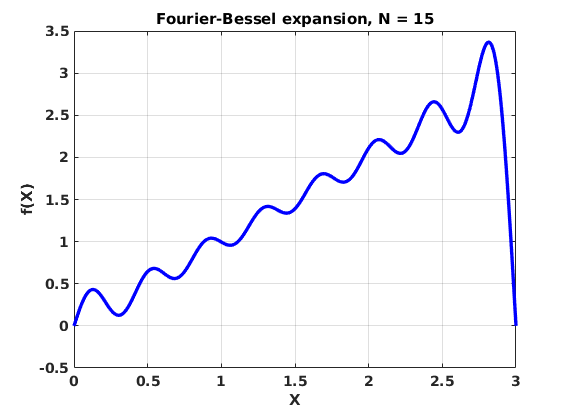
\includegraphics{lec19_ex1_N15.png}
\caption{Fourier-Bessel expansion of $f(x)=x$.}
\label{fig:lec19-ex1-n15}
\end{marginfigure}
The Fourier-Bessel expansion of $f(x)=x$ with $N=15$ is shown in Figure \ref{fig:lec19-ex1-n15}.  Note that the expansion for $N=15$ looks pretty rough. There are many wiggles through the domain and the expansion drops suddenly to zero as the function approaches $x=3$.  The reason for this is that \emph{it had to.}  We are building the expansion with orthogonal functions that are all equal to zero at $x=3$.  Of course $f(x)=x$ is equal to 3 at $x=3$ so something had to give.  

\begin{marginfigure}
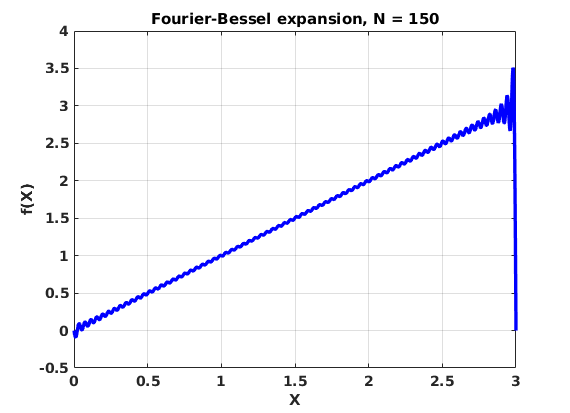
\includegraphics{lec19_ex1_N150.png}
\caption{Fourier-Bessel expansion of $f(x)=x$.}
\label{fig:lec19-ex1-n150}
\end{marginfigure}
We can improve the quality of the expansion by taking more terms.  Luckily, since we are using a computer, it is no problem at all to simply increase $N$; the computer does the same thing, just more of it.  The result is shown in Figure \ref{fig:lec19-ex1-n150} where the wiggliness remains---including the Gibbs phenomena we saw with Fourier series---but overall the representation is much more exact.

\section{Measuring Expansion Accuracy}
There is a straight-forward way to be more precise when we speak of the accuracy of an orthogonal function expansion.  A frequently used relative error measure is shown in Equation \ref{eq:lec19-rel-err}:

\begin{multline}
\text{Relative error} = \frac{\left(f(x) - FB(x), f(x)-FB(x)\right)}{\left(f(x),f(x)\right)} = \cdots \\ \frac{\int_a^b \left(f(x)-FB(x)\right)^2 \ dx}{\int_a^b f(x)^2 \ dx}
\label{eq:lec19-rel-err}
\end{multline}
\begin{marginfigure}
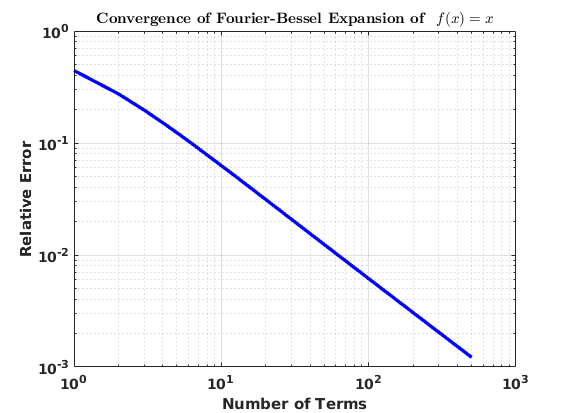
\includegraphics{lec19_ex1_converge.png}
\caption{Convergence of the Fourier-Bessel expansion of $f(x)=x$.}
\label{fig:lec19-converge}
\end{marginfigure}
MATLAB code for quantitatively measuring the relative error as the number of terms increases is shown below.  From Figure \ref{fig:lec19-converge} we can see that, as expected, the relative error steadily goes down.\sidenote{Note that it is conventional to show convergence graphs such as this on a log-log plot.  Eventually, we should expect errors in the determination of Bessel function roots and/or errors in carrying out the numeric integration to prevent further reduction in relative error.} 
%\begin{fullwidth}
\begin{lstlisting}[name=lec19-converge,style=myMatlab]
clear
clc
close 'all'

N = 500; % number of eigenvalues
a = 0; b = 3; % bounds of the domain
nu = 1; kind = 1;
k = besselzero(nu,N,kind); % get roots
alpha = k/b;

f = @(x) x; 
cn = nan(N,1); % store the coefficients (optional)
rel_err = nan(N,1); 

FB = @(x) 0; % initialize the Fourier-Bessel expansion
for n = 1:N
    % compute the i-th coefficient
    cn(n) =...
        integral(@(x) f(x).*besselj(nu,alpha(n)*x).*x,a,b)./...
        integral(@(x) x.*besselj(nu,alpha(n)*x).^2,a,b);
    % update the Fourier-Bessel expansion
    FB = @(x) FB(x) + cn(n)*besselj(nu,alpha(n)*x);

    % calculate sqruare norm of the relative "error"
    err_fn = @(x) FB(x) - f(x); 
    rel_err(n) = integral(@(x) err_fn(x).^2,a,b)./...
        integral(@(x) f(x).^2,a,b); 
end

figure(1)
loglog(1:N,rel_err,'-b',...
    'LineWidth',3);
title('\textbf{Convergence of Fourier-Bessel Expansion of } $$f(x)=x$$',...
    'Interpreter','latex');
ylabel('Relative Error','FontSize',14,...
    'FontWeight','bold');
xlabel('Number of Terms','FontSize',14,...
    'FontWeight','bold');
grid on
set(gca,'FontSize',12,'FontWeight','bold');
\end{lstlisting}
%\end{fullwidth}


